\documentclass[10pt]{article}

\usepackage[T1]{fontenc}
\usepackage[utf8]{inputenc}
%\usepackage{beton}
%\usepackage{ccfonts}
%\usepackage{concrete}
\usepackage{concmath}
\usepackage{eulervm}
\usepackage{amsmath,amsthm,amssymb}
\usepackage{mathtools}
\usepackage{multicol}
\usepackage{marginnote}
\usepackage{pgfplots}
\usepackage{float}
\usepackage{hyperref}
\usepackage{bbm}
\usepackage{booktabs}
\pgfplotsset{compat=1.5}

\usepackage{listings}
\usepackage{xcolor}
\definecolor{codegreen}{rgb}{0,0.6,0}
\definecolor{codegray}{rgb}{0.5,0.5,0.5}
\definecolor{codepurple}{rgb}{0.58,0,0.82}
\definecolor{backcolour}{rgb}{0.95,0.95,0.92}
\lstdefinestyle{mystyle}{
    backgroundcolor=\color{backcolour},   
    commentstyle=\color{codegreen},
    keywordstyle=\color{magenta},
    numberstyle=\tiny\color{codegray},
    stringstyle=\color{codepurple},
    basicstyle=\ttfamily\footnotesize,
    breakatwhitespace=false,         
    breaklines=true,                 
    captionpos=b,                    
    keepspaces=true,                 
    numbers=left,                    
    numbersep=5pt,                  
    showspaces=false,                
    showstringspaces=false,
    showtabs=false,                  
    tabsize=2
}

\lstset{language=Python, style=mystyle}

\usepackage{mathtools}

\usepackage{wasysym}
\usepackage[margin=1.5in]{geometry} 
\usepackage{enumerate}
\index{\usepackage}\usepackage{multicol}

\newcommand{\N}{\mathbf{N}}
\newcommand{\Z}{\mathbb{Z}}

\newcommand{\R}{\mathbf{R}}
\newcommand{\C}{\mathbf{C}}
\newcommand{\Pbb}{\mathbb{P}}
\newcommand{\Fcal}{\mathcal{F}}
\newcommand{\Acal}{\mathcal{A}}
\newcommand{\Ecal}{\mathcal{E}}
\newcommand{\Ebb}{\mathbb{E}}
\newcommand{\Qbb}{\mathbb{Q}}


\renewcommand{\mathbf}{\mathbold}

\newenvironment{theorem}[2][Theorem]{\begin{trivlist}
  \item[\hskip \labelsep {\bfseries #1}\hskip \labelsep {\bfseries #2.}]}{\end{trivlist}}
\newenvironment{lemma}[2][Lemma]{\begin{trivlist}
  \item[\hskip \labelsep {\bfseries #1}\hskip \labelsep {\bfseries #2.}]}{\end{trivlist}}
\newenvironment{exercise}[2][Exercise]{\begin{trivlist}
  \item[\hskip \labelsep {\bfseries #1}\hskip \labelsep {\bfseries #2.}]}{\end{trivlist}}
\newenvironment{reflection}[2][Reflection]{\begin{trivlist}
  \item[\hskip \labelsep {\bfseries #1}\hskip \labelsep {\bfseries #2.}]}{\end{trivlist}}
\newenvironment{proposition}[2][Proposition]{\begin{trivlist}
  \item[\hskip \labelsep {\bfseries #1}\hskip \labelsep {\bfseries #2.}]}{\end{trivlist}}
\newenvironment{corollary}[2][Corollary]{\begin{trivlist}
  \item[\hskip \labelsep {\bfseries #1}\hskip \labelsep {\bfseries #2.}]}{\end{trivlist}}

\newenvironment{definition}[2][Definition]{\begin{trivlist}
  \item[\hskip \labelsep {\bfseries #1}\hskip \labelsep {\bfseries #2.}]}{\end{trivlist}}

\begin{document}
	
  \renewcommand{\qedsymbol}{\smiley}
	\title{Investments Class \\ Problem set 1}
	\author{Daniel Grosu, William Martin, Denis Steffen}
	
	\maketitle

  \begin{exercise}{1}(Utility Theory)

From the statement, we know that the random variables $Y$ and $\epsilon$ have the following distributions:
$$ Y \sim \mathcal{N}(\mu_Y,\sigma_Y^2), \quad \epsilon \sim \mathcal{N}(-\mu_\epsilon,\sigma_\epsilon^2)$$ but they are not independent and have correlation $\rho$. 
The covariance between the two is $Cov(Y,\epsilon) = \rho\sqrt{\sigma_Y^2}\sqrt{\sigma_\epsilon^2} = \rho\sigma_\epsilon\sigma_\epsilon$. 

We have to consider the random vector $\mathbf{Z} = (Y,\epsilon)^\top$ which has multivariate gaussian distribution because every linear combination of the components $\alpha Y + \beta \epsilon$ is normally distributed. Thus:
$$ \mathbf{Z} \sim \mathcal{N}_2 \left( {\mu_Y \choose -\mu_\epsilon},\begin{bmatrix}
  \sigma^2_Y&\rho\sigma_Y\sigma_\epsilon\\
  \rho\sigma_Y\sigma_\epsilon&\sigma_\epsilon^2\\
  \end{bmatrix} \right) $$

  First, we can calculate the relative risk aversion and the absolute risk aversion:
\begin{equation*}
  \text{ARA}(W) = -\frac{u''(W)}{u'(W)} = \frac{a^2e^{-aW}}{ae^{-aW}} = a, \quad \text{RRA}(W) = -\frac{Wu''(W)}{u'(W)} = -aW
\end{equation*} since $u'(W) = ae^{-aW}$ and $u''(W) = -a^2e^{-aW}$.

Then, we want to compute the insurance premium $\pi$ to insure the risk of $\epsilon$ such that: $$ \Ebb[u(Y+\epsilon)] = \Ebb[u(Y-\pi)] $$
We can first compute the right hand side expectation using the moments generating function of a multivariate gaussian random variable $\mathcal{N}_n(\mathbf{\mu},\mathbf{\Sigma}) $:
$$ MGF_\mathbf{X}(t) = \Ebb[e^{\mathbf{t}^\top\mathbf{Z}}] = \exp(\mathbf{t}^\top\mathbf{\mu} + \frac{1}{2}\mathbf{t}^\top\mathbf{\Sigma}\mathbf{t})$$
Thus, 
\begin{align*}
  \Ebb[e^{-a(Y+\epsilon)}] = \Ebb[e^{-a\mathbbm{1}^\top\mathbf{Z}}] &= \exp(-a\mathbbm{1}^\top\mu + \frac{1}{2}a^2\mathbbm{1}^\top\mathbf{\Sigma}\mathbbm{1}) \\
  &= \exp(-a(\mu_Y - \mu_\epsilon)+\frac{1}{2}a^2(\sigma_Y^2 + 2\rho\sigma_Y\sigma_\epsilon + \sigma_\epsilon^2))
\end{align*}

On the other side, we can see that:
\begin{align*}
  \Ebb[e^{-a(Y-\pi)}] &= e^{a\pi}\Ebb[e^{-aY}] \\
  &= e^{a\pi}e^{-a\mu_Y + \frac{1}{2}a^2\sigma_Y^2}
\end{align*}
 
Combining the two, we get:
\begin{align*}
  &e^{-a(\mu_Y-\mu_\epsilon) +\frac{1}{2}a^2(\sigma_Y^2 + 2\rho\sigma_Y\sigma_\epsilon + \sigma_\epsilon^2)} = e^{a\pi}e^{-a\mu_Y + \frac{1}{2}a^2\sigma_Y^2}\\
  &\iff e^{a\pi} = e^{a\mu_\epsilon +\frac{1}{2}a^2(2\rho\sigma_Y\sigma_\epsilon + \sigma_\epsilon^2)}\\
  &\iff \pi = \mu_\epsilon + \frac{1}{2}a(2\rho\sigma_Y\sigma_\epsilon + \sigma_\epsilon^2)
\end{align*}
Finally, the maximum insurance premium we are willing to pay to insure the risk of $\epsilon$ is $\mu_\epsilon + \frac{1}{2}a(2\rho\sigma_Y\sigma_\epsilon + \sigma_\epsilon^2)$.

Furthermore, we can study how the premium evolves according to the five parameters of the random variable distributions. 
We differentiate $\pi$ with respect to these variables:
\begin{itemize}
  \item $\frac{\partial\pi}{\partial\mu_\epsilon} = 1$
  \item $\frac{\partial\pi}{\partial a} = \rho\sigma_Y\sigma_\epsilon + \sigma_\epsilon^2$
  \item $\frac{\partial\pi}{\partial\rho} = a\sigma_Y\sigma_\epsilon$
  \item $\frac{\partial\pi}{\partial\sigma_\epsilon} = a\rho\sigma_Y + \sigma_\epsilon$
  \item $\frac{\partial\pi}{\partial\sigma_Y} = a\rho\sigma_\epsilon$
\end{itemize}

  \end{exercise}


\begin{exercise}{2}(Value at Risk, Expected Shortfall, and Expected Utility)
  \begin{enumerate}[(a)]
    \item
  In order to compute the moments of the given distribution, one can use the
  built-in \textrm{NumPy} and \textrm{SciPy} functionality for samples. It is
  easy to see that by creating a sample in which the prior probabilities are the
  same as the ones given, the sample and the distribution moments will be the
  same. This is, however, only applicable for discrete distributions.
  \begin{lstlisting}
#%% Imports

import pandas as pd;
import numpy as np;
import matplotlib.pyplot as plt;

import scipy.stats as stats;

#%% Generating the Sample

pr = np.array([0.025, 0.05, 0.10, 0.10, 0.10, 0.2, 0.2, 0.2, 0.025]);
ret = np.array([-0.4, -0.2, -0.1, 0, 0.05, 0.1, 0.15, 0.20, 0.30]);


sample = np.array([]);

# Generate the sample with the given priors
for i in range(pr.size):
    # print(pr[i]);
    for j in range(int(1000*pr[i])):
        sample = np.append(sample, ret[i])


#%% Plotting the sample (visualization)

plt.figure();
plt.hist(sample);
plt.show();


#%% Sub-item (a): Compute the moments of the distribution

print(round(np.mean(sample), 3))
print(round(np.std(sample), 3))
print(round(stats.skew(sample), 3))
print(round(stats.kurtosis(sample), 3))
  \end{lstlisting}
  As such, the computed values are:

  \begin{figure}[H]
    \centering
    \begin{tabular}{|c | c |}
      \hline
      $\mu$ & 0.072 \\ \hline
      $\sigma$ & 0.137 \\ \hline
      g & -1.323 \\ \hline
      k &  1.953 \\\hline
    \end{tabular}
    \caption{The moments of the distribution}
  \end{figure}

  From the moments, we observe that the mean of the distribution is positive,
  but the distribution is negatively-skewed. For example, the lowest (negative)
  return is bigger in absolute value than the highest possible positive return.
  The kurtosis of any univariate normal distribution is 3. \textit{Excess
    kurtosis} is defined as the kurtosis minus 3. In our case the excess
  kurtosis is negative which classifies this distribution as a
  \textit{platykurtic} or sometimes called sub-Gaussian distribution. This means
  that the tales are thinner and sampling from it produces fewer and less
  extreme outliers than does the normal distribution.
\item
  The Value-at-Risk $VAR_p$ is the loss $l$ such that the probability of a loss
  higher than $l$ is bounded by $p$. For our discrete distribution this
  equivalent to the quantile for which the left tail has a total probability of
  $p$. For a discrete distribution, the values at risk are also discrete and as
  $p$ increases from $0$ to $1$, the $VAR$ increases when sum of the left prefix
  of the probabilities (left tail) becomes smaller than $p$. As such, $VAR_{1\%}
  = -.40 \times \$ 100 = -\$ 40$
  and $VAR_{5\%} = -.20 \times \$ 100 = -\$20$ because $1\% < 0.025$ and $0.025 < 5\% < 0.075$.

 \item
   By definition, the Expected Shortfall (ES) or the Conditional Tail
   Expectation (CTE) is the mean of the values at risk with probability smaller
   than $p$:
   \begin{equation*}
     ES_p = \frac 1 p \int_0^p VAR_\gamma d\gamma
   \end{equation*}
   For the distribution of asset returns it holds that:
   \begin{equation*}
     VAR_\gamma = \begin{cases} -\$ 40 & \gamma < 0.025 \\ -\$ 20 & 0.025 < \gamma < 0.075 \end{cases}
   \end{equation*}

   Hence, the Expected Shortfall at $5\%$ equals:
   \begin{equation*}
     ES_{5\%} = \frac{1}{5\%} \int_0^{5\%} VAR_\gamma d\gamma = \frac{1}{5\%} \left( 0.025 \times (-\$ 40) + 0.025 \times (-\$20) \right) = - \$ 30.
   \end{equation*}

   \item
     The break-even risk-free rate can be computed by equating the utility of
     the two scenarios: portfolio with all wealth invested in the risky asset
     or the risk-free rate:
     \begin{equation*}
       \Ebb \big[ u\left((1 + r) \times W_0\right) \big] = u(r_f \times W_0)
     \end{equation*}
     where the Constant Elasticity of Substitution (CES) utility function is
     \begin{equation*}
       u(c) = \frac{c^{1 - \gamma}}{1 - \gamma}, \;\; \gamma = 2
     \end{equation*}
     Solving for $r_f$:
     \begin{equation*}
       r_f = \frac{u^{-1}\left( \Ebb\big[ u\left( (1+r) \times W_0 \right) \big] \right)}{W_0}
     \end{equation*}

     The following Python code computes the equivalent risk-free rate to stand
     at $r_f = 5.03\%$. That is, given the customer's risk-averseness, he would
     be willing to forgo $\mu - r_f = 2.22\%$ in expected return if the risk
     is eliminated. The level of risk-free rate above which she would choose to
     invest all her wealth in the risk-free asset is $5.03 \%$. This cut-off
     rate decreases with the increase in the risk-aversion coefficient:
     \begin{figure}[H]
       \centering
          \begin{tabular}{||c|c||}
          \toprule
          $\gamma$ &        $r_f$ \\
          \midrule
          2  &       5.03\% \\ \hline
          3  &       3.59\% \\ \hline
          4  &       1.87\% \\ \hline
          5  &      -0.14\% \\ \hline
          6  &      -2.46\% \\ \hline
          7  &      -5.01\% \\ \hline
          8  &      -7.68\% \\ \hline
          9  &     -10.34\% \\ \hline
          10 &     -12.88\% \\ \hline
          11 &     -15.21\% \\ \hline
          12 &     -17.31\% \\ \hline
          13 &     -19.16\% \\ \hline
          14 &     -20.79\% \\ \hline
          \bottomrule
          \end{tabular}
      \end{figure}
      The break-even rate decreases because the investor becomes more
      risk-averse which translates into a lower risk-free rate that he would
      accept just to eliminate any risk.
    \begin{lstlisting}
#%% Part (d) Utility

def utility(w, gamma = 2):
    return np.power(w, 1 - gamma)/(1 - gamma)

def inverse_utility(u, gamma = 2):
    return np.exp(np.log(u*(1 - gamma))/(1 - gamma))


# Test the inverse utility function
# print(inverse_utility(utility(400)));

# 100% either in risky or risk-free

gamma_range = range(2, 15)
rf = pd.Series(data = np.zeros(len(gamma_range)),
               index = gamma_range,
               name = "rate")

W0 = 100

rf = [inverse_utility(np.mean([utility((1 + x) * W0, ra) for x in sample]), ra)/W0 - 1 for ra in gamma_range]
"""
for ra in gamma_range:
    expected_utility = np.mean([utility((1 + x) * W0, ra) for x in sample])
    rf[ra] = inverse_utility(expected_utility, ra) / W0 - 1
"""
    
pf = pd.DataFrame(data = rf, index = gamma_range)
pf.columns = ['rate']
display(pf.style.format({"rate": lambda x: "{:.2%}".format(x)}))

print('The breakeven risk-free asset is %.2f%%' % (pf.loc[2] * 100))

print('The investor is willing to forgo %.2f%% in expected return' % ((mu - pf.loc[2])*100))
    \end{lstlisting}
    \item
      If she can invest a fraction of her wealth in the risk-free asset, the
      rate at which she will not choose to invest anything in the risk-free
      asset is between $2\%$ and $2.5\%$ which is lower than the risk-free rate
      found in the previous sub-item.
      While the $r_f = 5.03\%$ risk-free rate generates the same amount of
      utility as the risky asset alone, the two combined is able to produce more
      utility because the investor compromises between return and risk by
      investing in the risk-less asset and mitigating the unattractive risk.
      At the same time, the investor will choose not to invest in the risk-free
      rate if its rate is too disadvantageous and will choose to invest all of
      its wealth in the risk-less asset if its return is at least the expected
      return of the risky asset.

      The rate at which she will not choose to
      invest anything in the risk-free asset is lower than the risk-free rate
      found in the previous sub-item because if it were higher or equal ($r'_f \geq 
      r_f$), by
      choosing not to invest in it at all, the utility generated will be
      $\Ebb\left[ (1 + r) \times W_0 \right]$ while she could have generated more
      utility by simply investing all $W_0$ in the risk-free rate:
      $u(r'_f \times W_0) \geq u(r_f \times W_0) = \Ebb\left[ (1 + r) \times W_0
      \right]$, hence contradiction.
      
\begin{lstlisting}
#%% Part (e)

gamma = 2;
# Start investing all the wealth in the risk-less asset at approx 7.2% return
# it is higher than the equivalent risk-free interest rate providing the same
# utility as the expectation of the utility of the risky return.

rf_range = np.arange(0.000, 0.074, 0.005)

pi_star = pd.Series(data = None, index = rf_range, name = "Pi*")

for rf in rf_range:
    utility_pi = {};
    # invest pi in the risk-less assets
    for pi in np.arange(0, 1 + 0.05, 0.05):
        
        utility_pi[pi] = np.mean([utility((1 + x) * W0 * (1 - pi) +
                              (1 + rf) * W0 * pi, gamma) for x in sample]);
    pi_star[rf] = max(utility_pi, key = utility_pi.get);
    
display(pi_star)

#%%

plt.figure()
plt.plot(pi_star)
plt.show()

pi = pd.DataFrame(data = pi_star, index = rf_range)
pi.index.names = ['rf']

display(pi.style.format({"Pi*": lambda x: "{:.2}".format(x)}))
print(pi.to_latex(float_format=lambda x: '%10.2f' % (x*100)))

print('The breakeven risk-free asset is %.2f%%' % (pf.loc[2] * 100))

print('The investor is willing to forfeit %.2f%% in expected return' % ((mu - pf.loc[2])*100))


\end{lstlisting}


      \begin{figure}[H]
        \centering
       \begin{tabular}{||c|c||}
\toprule
$r_f$ &        $\pi^* \times 100\%$ \\
\midrule
0.000 &       0.00 \\ \hline
0.005 &       0.00 \\ \hline
0.010 &       0.00 \\ \hline
0.015 &       0.00 \\ \hline
0.020 &       0.00 \\ \hline
0.025 &       5.00 \\ \hline
0.030 &      10.00 \\ \hline
0.035 &      20.00 \\ \hline
0.040 &      30.00 \\ \hline
0.045 &      35.00 \\ \hline
0.050 &      45.00 \\ \hline
0.055 &      55.00 \\ \hline
0.060 &      70.00 \\ \hline
0.065 &      80.00 \\ \hline
0.070 &      95.00 \\ \hline
0.075 &      100.00 \\ \hline
\bottomrule
\end{tabular}
\caption{The optimal fraction of wealth to invest in the risk-free asset under
  various risk-free rates}

 
      \end{figure}

  \end{enumerate}

\newpage

\end{exercise}

	

\begin{exercise}{3}

	We compute the mean and variance of daily simple returns for the 5 companies at hand as well as the mean and variance of the 'winsorized' empirical distribution:
	
	\begin{table}[h!]
		\centering
 		\begin{tabular}{||c c c c c||} 
 		\hline
		& mean & 'winsorized' mean & variance & 'winsorized' variance \\ [0.5ex] 
 		\hline\hline
 		aapl & 0.001167 & 0.000705 & 0.000665 & 0.000262 \\ 
 		gs & 0.000437 & 0.000296 & 0.000547 & 0.000232 \\
 		msft & 0.000388 & 0.000309 & 0.000370 & 0.000192 \\
 		pg & 0.000306 & 0.000336 & 0.000177 & 0.000109 \\
 		ge & -9.246418e-05 & 4.680753e-05 & 0.000376 & 0.000184 \\ [1ex] 
 \hline
 \end{tabular}
	\end{table}
	
	Moreover, we plot and compare the density function of stock returns with the normal distributions with empirical mean and variance and empirical 'winsorized' mean and variance. We do this for all 5 companies:
	
		\begin{figure}[H]
	
			\centering
			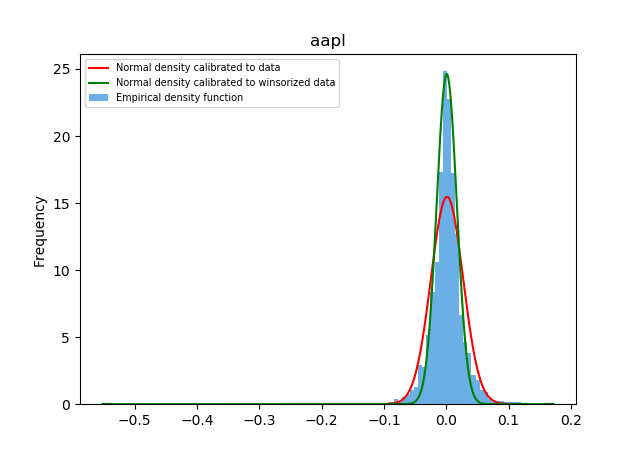
\includegraphics[scale=0.7]{Figures/ex3_aapl.png}	
			\caption{Density function of stock returns with empirical normal distributions (non-winsorized and winsorized) of aapl}	
			\label{fig:ex3_aapl}
	
		\end{figure}
		
		\begin{figure}[H]
	
			\centering
			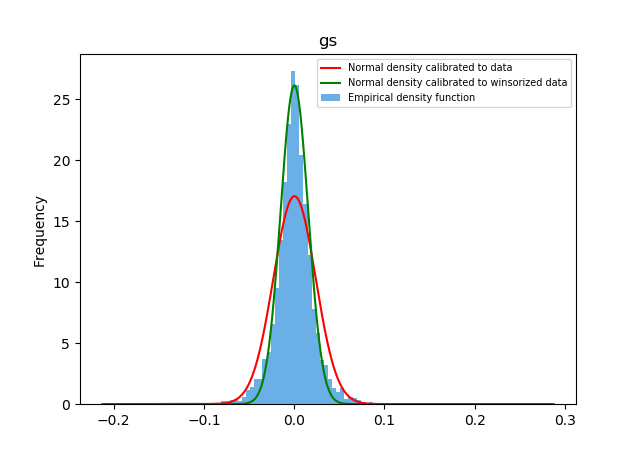
\includegraphics[scale=0.7]{Figures/ex3_gs.png}	
			\caption{Density function of stock returns with empirical normal distributions (non-winsorized and winsorized) of gs}	
			\label{fig:ex3_gs}
	
		\end{figure}
		
		\begin{figure}[H]
	
			\centering
			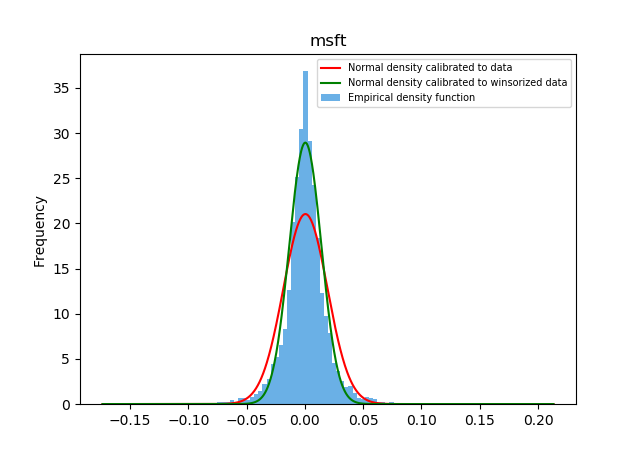
\includegraphics[scale=0.7]{Figures/ex3_msft.png}	
			\caption{Density function of stock returns with empirical normal distributions (non-winsorized and winsorized) of msft}	
			\label{fig:ex3_msft}
	
		\end{figure}
		
		\begin{figure}[H]
	
			\centering
			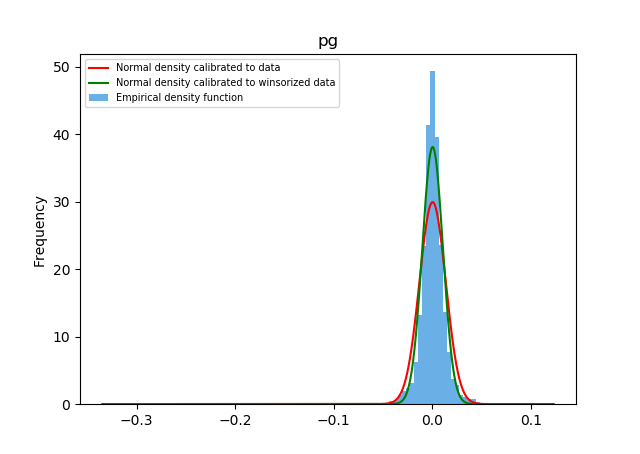
\includegraphics[scale=0.7]{Figures/ex3_pg.png}	
			\caption{Density function of stock returns with empirical normal distributions (non-winsorized and winsorized) of pg}	
			\label{fig:ex3_pg}
	
		\end{figure}
		
		\begin{figure}[H]
	
			\centering
			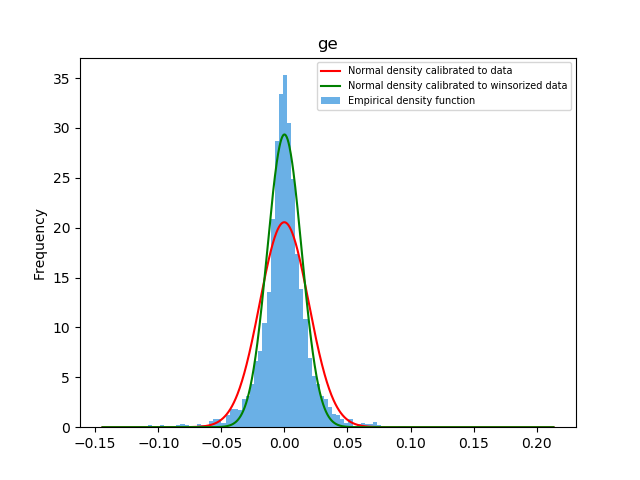
\includegraphics[scale=0.7]{Figures/ex3_ge.png}	
			\caption{Density function of stock returns with empirical normal distributions (non-winsorized and winsorized) of ge}	
			\label{fig:ex3_ge}
	
		\end{figure}

	For each stock, we compute the $95\%$ and $99\%$ Value-at-Risk from the empirical distribution of returns and compare the values with those of a normal distribution with corresponding mean and variance:
	
	\begin{table}[h!]
		\centering
 		\begin{tabular}{||c c c c c||} 
 		\hline
		& $95\%$ VaR (empirical) & $99\%$ VaR (empirical)  & $95\%$ VaR (normal) & $99\%$ VaR (normal) \\ [0.5ex] 
 		\hline\hline
 		aapl & -0.038023 & -0.064111 & -0.041281 & -0.058868 \\ 
 		gs & -0.033770 & -0.062409 & -0.038048 & -0.053993 \\
 		msft & -0.028345 & -0.054692 & -0.031273 & -0.044392 \\
 		pg & -0.017401 & -0.034385 & -0.021615 & -0.030697 \\
 		ge & -0.029225 & -0.056332 & -0.032028 & -0.045260 \\ [1ex] 
 \hline
 		\end{tabular}
	\end{table}

	We do the same for the Conditional Expected Shortfall:
	
	

\end{exercise}
  
\end{document}

